\subsection{System Design} \label{sec:system-design}
The \textit{Beerlytics} system is composed of multiple subsystems (Figure \ref{fig:architecture}).
These subsystems communicate with each other and provide downstream information which their dependent systems utilize for further work.
There are 4 primary servers involved: (1) the \textit{RateBeer} server, (2) a private server for data collection and database hosting (Section \ref{sec:data-collection}), (3) the computation server (Section \ref{sec:data-analysis}), and (4) the frontend server which runs the API.
In order to evaluate the proposed system's effectiveness through user testing (Section \ref{sec:evaluation}) a frontend prototype is implemented as a web application.
The application runs inside a web browser on the user's device and communicates with the API using the HTTP protocol.
First, the API is explained in section \ref{sec:api} which is followed by section \ref{sec:frontend-prototype} covering the frontend prototype more thoroughly. 

\begin{figure}[h]
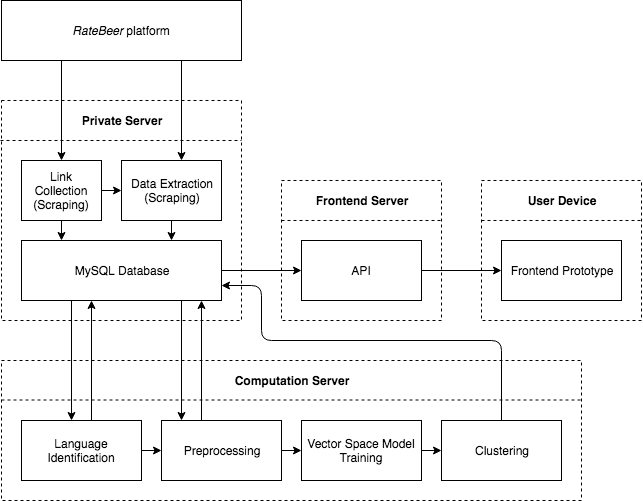
\includegraphics[width=8cm]{assets/architecture.png}
\caption{Beerlytics system architecture diagram}
\centering
\label{fig:architecture}
\end{figure}

\subsubsection{API} \label{sec:api}
The API acts as the central communication gateway between the private database server and the frontend prototype (Figure \ref{fig:architecture}).
It is implemented in JavaScript using the Node.js \cite{Tilkov2010} runtime and relies on \textit{micro}\footnote{\url{https://github.com/zeit/micro}, accessed: 17-07-2018} as a HTTP microservice framework. 
Each API endpoint serves a specific purpose for the frontend prototype (Table \ref{tbl:api-endpoints}).

\begin{table}[h]
    \centering
    \begin{tabular}{ l p{0.5\linewidth} }
        \hline
        \emph{Route} & \emph{Purpose} \\
        \hline
        /search/(:query) & Most popular beers without query or search beer by name \\
        /beer/:id/nn & Nearest neighbor keyword insights for a beer \\
        /beer/:id/places & Locations of a beer's distribution places \\
        /beer/:id/reviews & Reviews of a beer grouped by word embedding algorithms \\
        /beer/:id & Metadata about a beer, e.g., name and description \\
        /user/:id/locations & Locations of a user's reviewed beers \\
        \hline
    \end{tabular}
    \caption{API endpoints and purposes} \label{tbl:api-endpoints}
\end{table}

The following paragraphs shortly discuss the available endpoints:

\noindent
\textbf{Search:} Its route contains an optional query parameter.
Depending on the presence of the query parameter the endpoint switches behavior.
Provided no query parameter is present the API returns a list of the 16 most popular beers ordered by the count of their total ratings.
Given a query, all beers are searched by their name and sorted according to the relevance towards the query.
The search index is generated by the \textit{Lunr.js}\footnote{\url{https://github.com/olivernn/lunr.js}, accessed: 17-07-2018} full-text search library.

\noindent
\textbf{Beer Nearest Neighbors:} This endpoint returns the nearest neighbor terms per word embedding and query term as computed in section \ref{sec:data-analysis} using the k-NN algorithm.
The similarity for neighboring terms is a percentage decimal between 0 and 1.
As the words in the database are in their stemmed form (see section \ref{sec:preprocessing}) the token dictionary enables a translation back to a list of original words (Table \ref{tbl:schema.token_dictionary}).

\noindent
\textbf{Beer Places}: Gathers geocoordinates (latitude, longitude) of all places selling a specific beer.
These coordinates are lazily geocoded from the address information captured from \textit{RateBeer}.
Google provides a geocoding service\footnote{\url{https://developers.google.com/maps/documentation/javascript/geocoding}, accessed: 17-07-2018} which is used to translate a place's address into geocoordinates if it has not been geocoded before.

\noindent
\textbf{Beer Reviews:} The review cluster information computed during data analysis (Section \ref{sec:data-analysis}) using the k-means algorithm is retrieved by this endpoint.
It loads all review centroids per word embedding algorithm for a specific beer.

\noindent
\textbf{Beer Metadata:} Returns static metadata about a beer (e.g., name, image, description) as scraped from its \textit{RateBeer} page.
It also computes the average rating using all reviews of a beer.

\noindent
\textbf{User Locations:} Similar to the beer nearest neighbors endpoint as it also lazily geocodes addresses into geocoordinates.
It gathers all beers which have been reviewed by a specific user and returns a list of their respective locations.


\subsubsection{Frontend Prototype} \label{sec:frontend-prototype}
The frontend prototype is a JavaScript application based on modern frameworks.
\textit{Nuxt.js}\footnote{\url{https://nuxtjs.org/}, accessed: 17-07-2018} for component-based application development and \textit{Bulma}\footnote{\url{https://bulma.io/}} as a CSS\footnote{\url{https://www.w3.org/Style/CSS/Overview.en.html}, accessed: 17-07-2018} framework which provides basic styling.
It uses asynchronous HTTP requests to communicate with the API backend (Section \ref{sec:api}).
The various components of the frontend prototype fulfill their specific data requirements by sending requests to respective endpoints (Table \ref{tbl:api-endpoints}).

\begin{figure}[h]
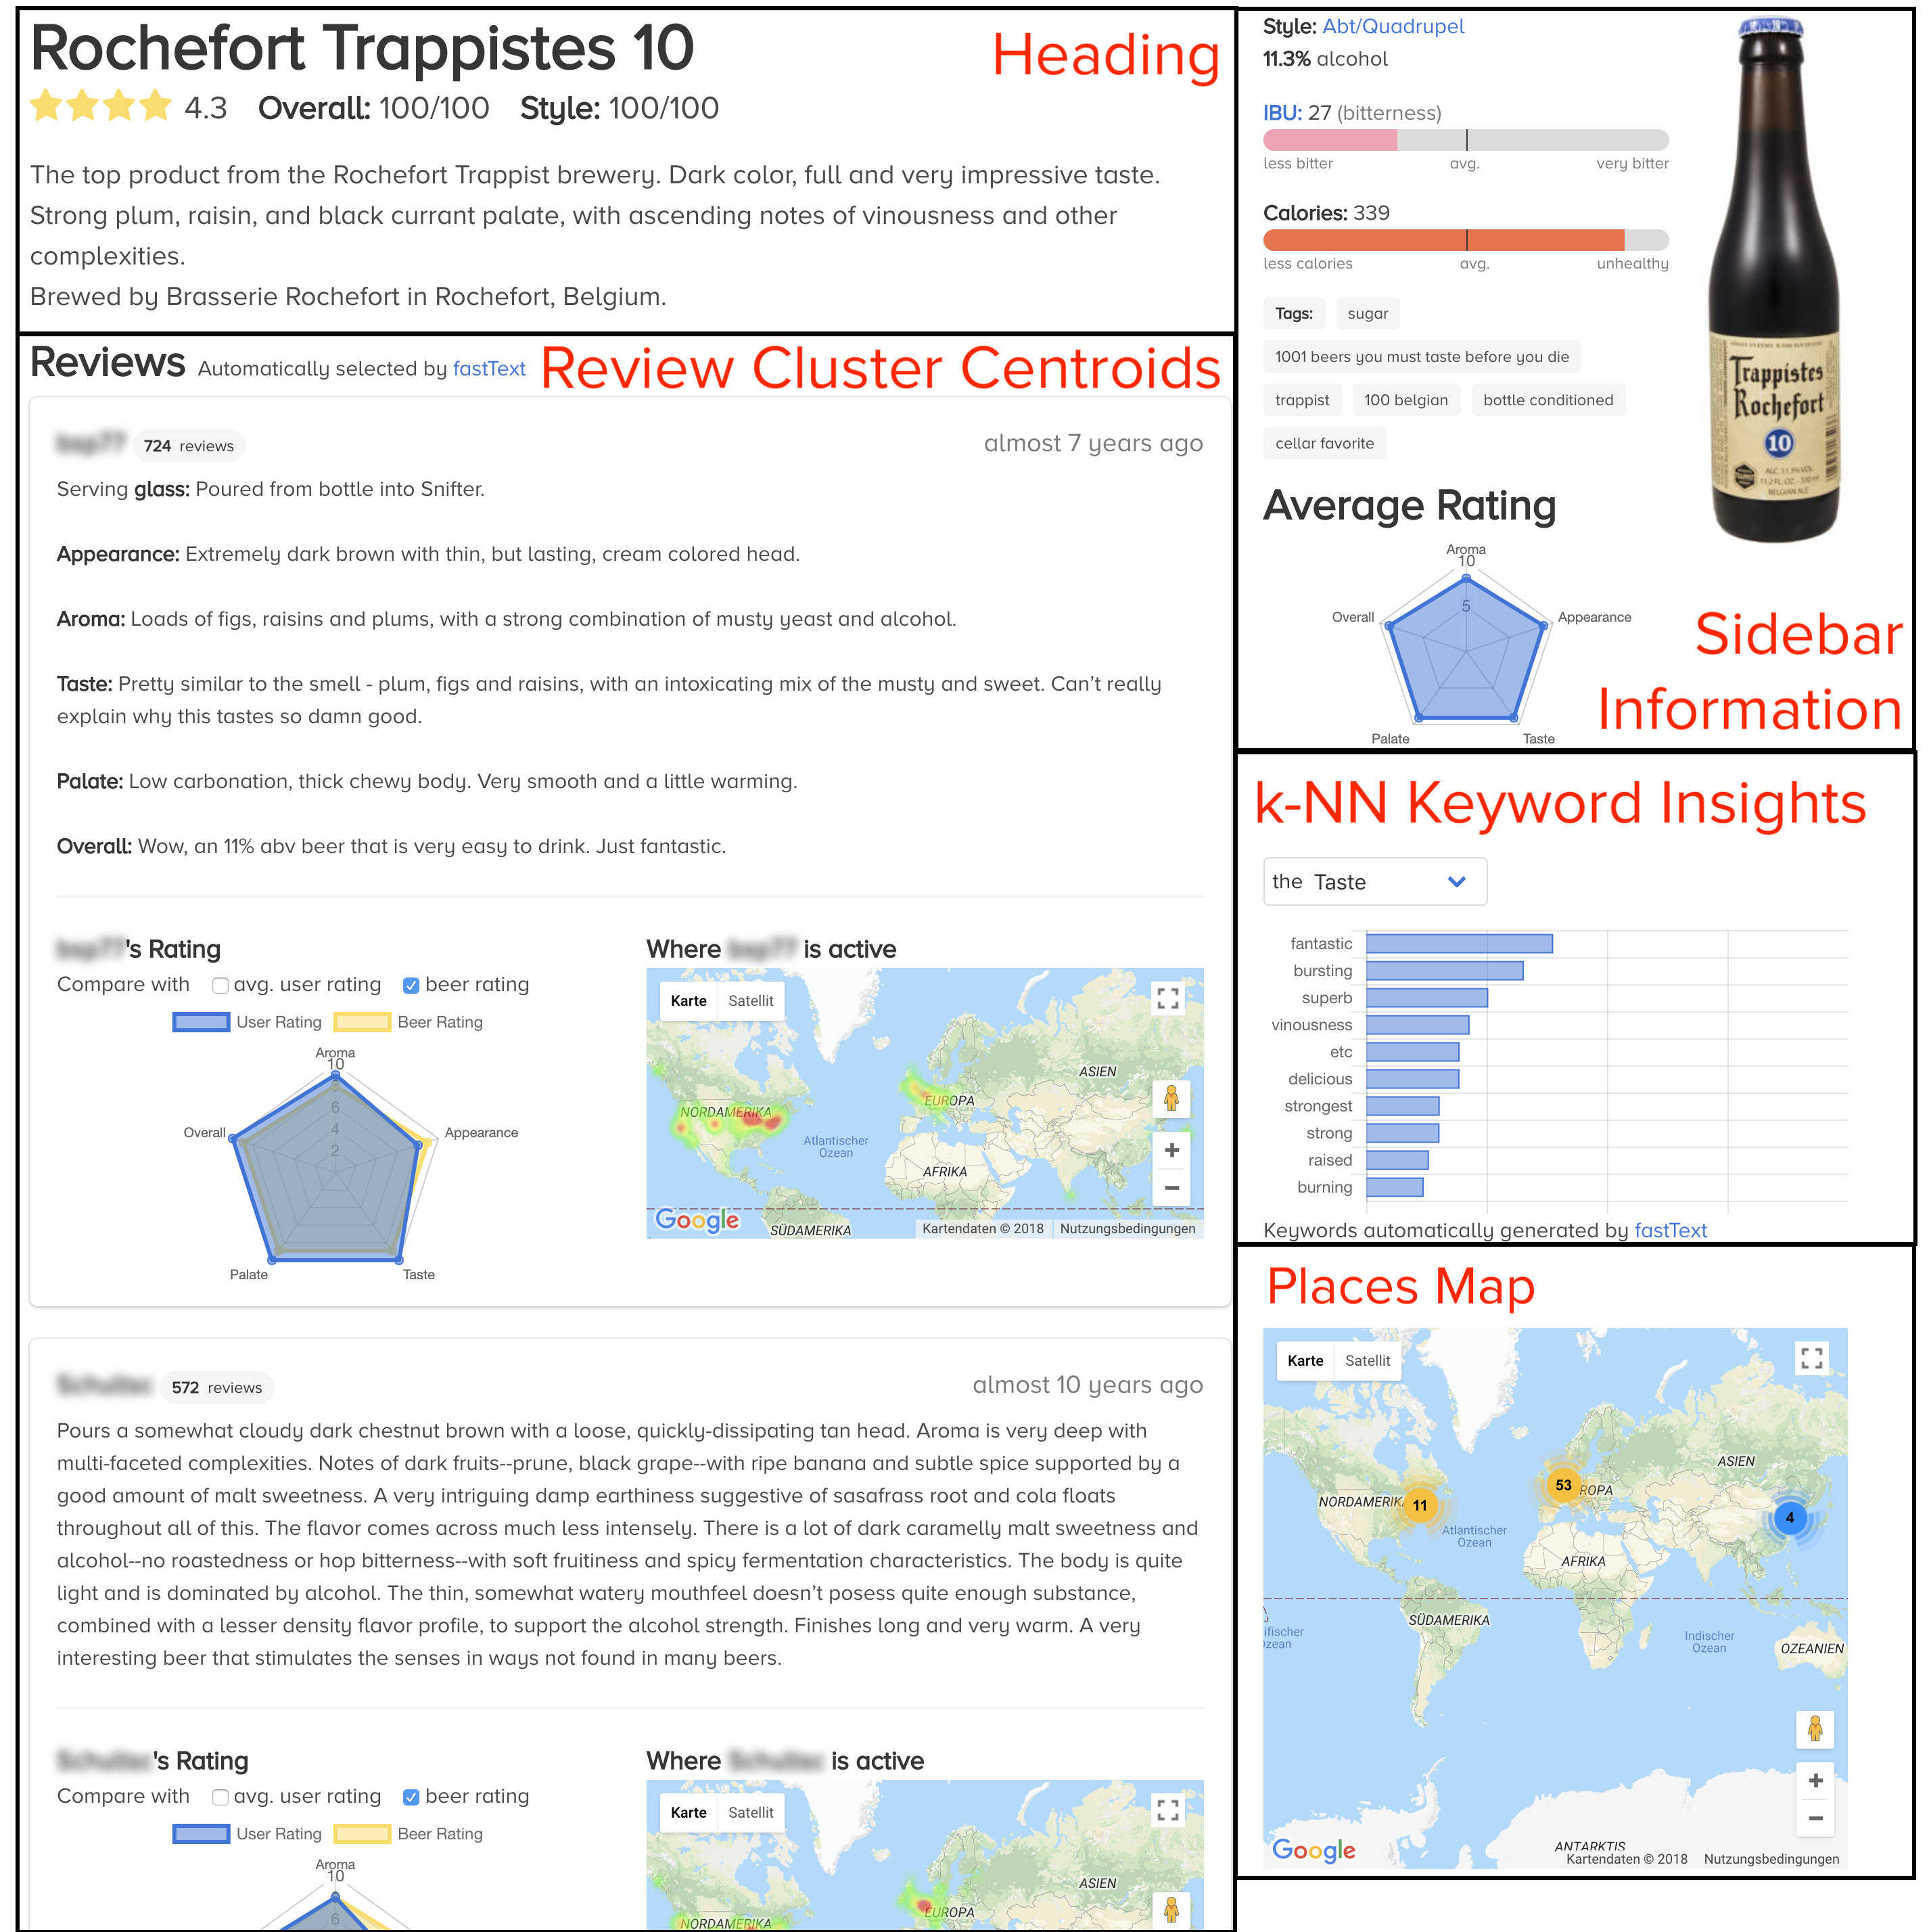
\includegraphics[width=8cm]{assets/beerlytics_components.png}
\caption{Components on the Beerlytics beer page}
\centering
\label{fig:beerlytics-components}
\end{figure}

A user's journey begins on the index page (Figure \ref{fig:beerlytics-index}) which features a prominent search bar and a list of beers.
Beers are displayed using their name, amount of ratings, and a star rating from 0 to 5 stars.
Typing into the search input automatically triggers search requests against the API's search endpoint.
The list is automatically updated using the search results sorted by relevance.

Clicking on a beer entry redirects the user to the corresponding beer detail page (Figure \ref{fig:beerlytics-beer}).
At the top of the page resides the heading component which renders static data as gathered from \textit{RateBeer} (Figure \ref{fig:beer-heading}).
It includes the beer's name, previously mentioned star rating, and scores ranging from 0 to 100 for the categories \textit{overall} and \textit{style}.
Below is the official description text provided by the brewery.
The description follows a sentence stating the brewery name and location.

Continuing the page downwards reveals the reviews component which takes up the remaining space of the primary content column (Figure \ref{fig:beer-review}).
This component is particularly interesting in the sense that it utilizes existing data from \textit{RateBeer} (such as username, review text, and user rating) and merges it with dynamic data computed by data analysis.
It restricts the set of visible reviews to the currently selected word embedding algorithm and is thereby only showing the cluster centroid reviews for this technique.
In order to educate the user about this behavior the heading of the reviews component contains a disclaimer stating:
\begin{quote}
\emph{``Reviews automatically selected by <word embedding algorithm>''}
\end{quote}
The bottom part of a review contains visual components working towards building a visual product story and supporting data comprehension of the user.
Instead of displaying a textual description of the user rating a radar chart is used to visualize the strength of each aspect.
Moreover, the radar chart allows overlaying the average rating of the current beer or the average rating of the review author (aggregated and averaged from all reviews authored by this user).
Next to the radar chart is a heat map which indicates the locations of all beers reviewed by the same author.
It essentially summarizes a user by visualizing their geospatial interest in relation to the reviewed beers.

\begin{figure}[b]
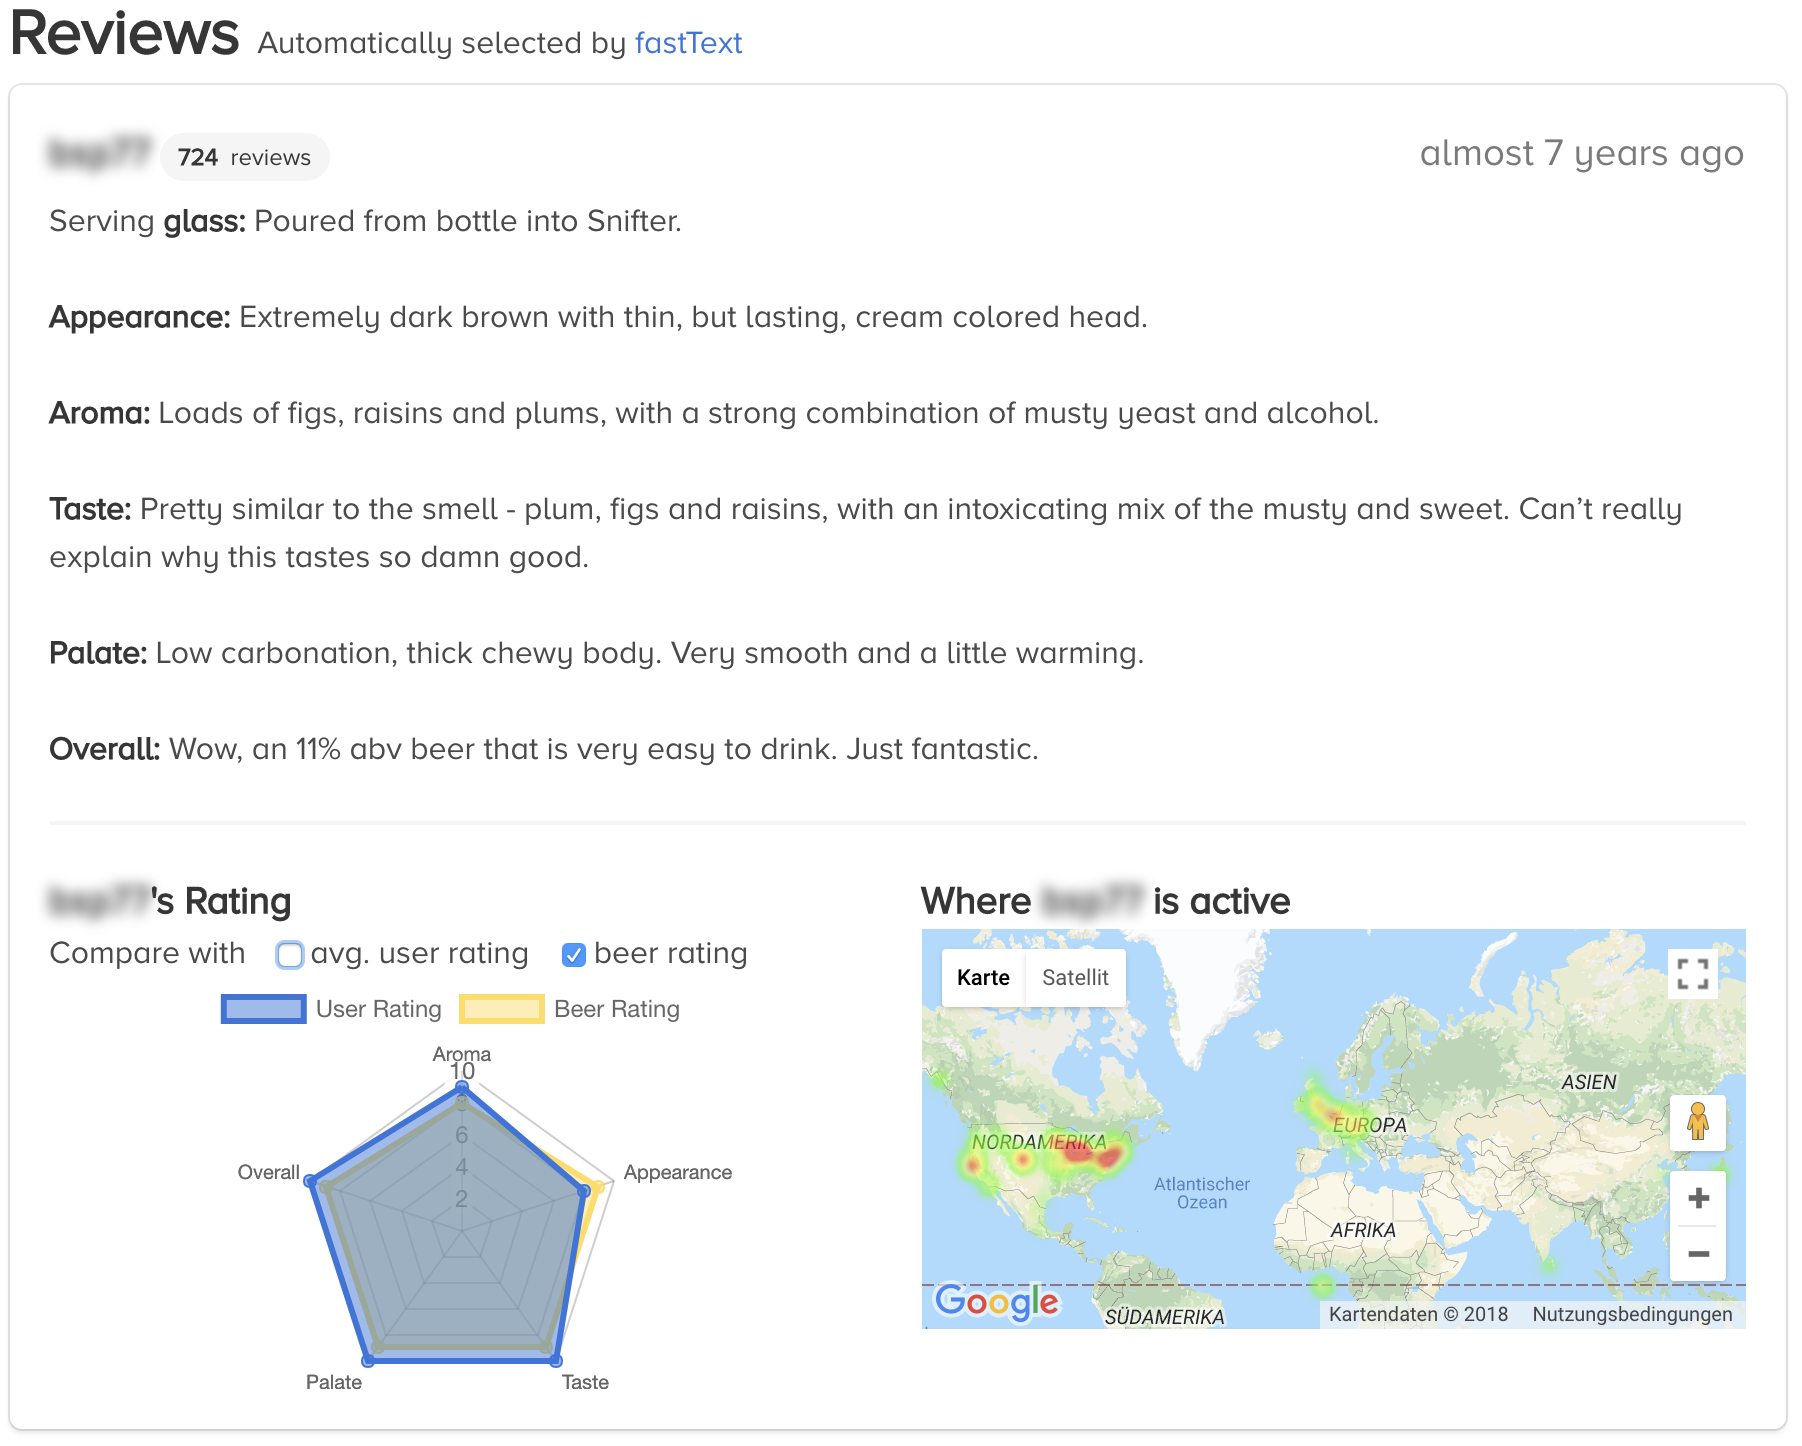
\includegraphics[width=5cm]{assets/beer_review.png}
\caption{User review on Beerlytics}
\centering
\label{fig:beer-review}
\end{figure}

The sidebar component provides factual information about the beer (Figure \ref{fig:beer-sidebar}).
Textual descriptions are used for the beer style and alcohol by volume (ABV) percentage with the beer style linking back to the corresponding \textit{RateBeer} page.
In contrast to that stand the scales for international bitterness units (IBU) and calories per serving below.
Displaying these measurements as simple values provide little to no use for users missing the appropriate background knowledge.
Therefore, employing scales creates the necessary context to judge where these values lay in comparison to other beers.
Labels below the scales annotate minimum, average, and maximum marks.
Furthermore, color gradients of the scale bar support cognition by featuring different colors and varying intensity in correlation to the underlying value.
The selected gradients are ensured to be safe for color blindness as they stem from the \textit{ColorBrewer2}\footnote{\url{http://colorbrewer2.org}, accessed: 05-07-2018} tool which provides color gradients for sequential, diverging, and qualitative data based on research \cite{Harrower2011}.
Users on \textit{RateBeer} crowdsource sets of tags for beers which reappear as a simple list of formatted links in this prototype.
Another radar chart concludes the bottom part of the sidebar information box which visualizes the aggregated, average rating of the current beer.
In comparison to the radar chart in a review component, this chart does not offer interactivity besides hovering on data points to inspect their precise value.

Beneath the previously discussed sidebar information is the keywords component or nearest neighbors visualization (Figure \ref{fig:beer-nn}).
Similarly to the reviews component, it builds on the result of the k-NN data analysis computation (Section \ref{sec:clustering}).
The visualization itself is a horizontal bar chart with the y-axis displaying neighboring terms.
Its x-axis does not have a legend annotating discrete values.
Intentionally hiding the x-axis legend is based on the assumption that users are not interested in reading similarity values in percent (This assumption is picked up again in section \ref{sec:results}).
Suppressing this information reduces noise and clutter on the page and emphasizes the length of bars in relation to each other.
The currently selected query keyword is selectable using a dropdown list above the bar chart.
This list contains the query terms as discussed in section \ref{sec:clustering}.
Switching the query keyword or selected word embedding algorithm automatically adapts the displayed neighboring terms in the bar chart.
In accordance with the disclaimer in the reviews component, another annotation below the visualization states: 
\begin{quote}
\emph{``Keywords automatically generated by <word embedding algorithm>''}
\end{quote}

\begin{figure}[t]
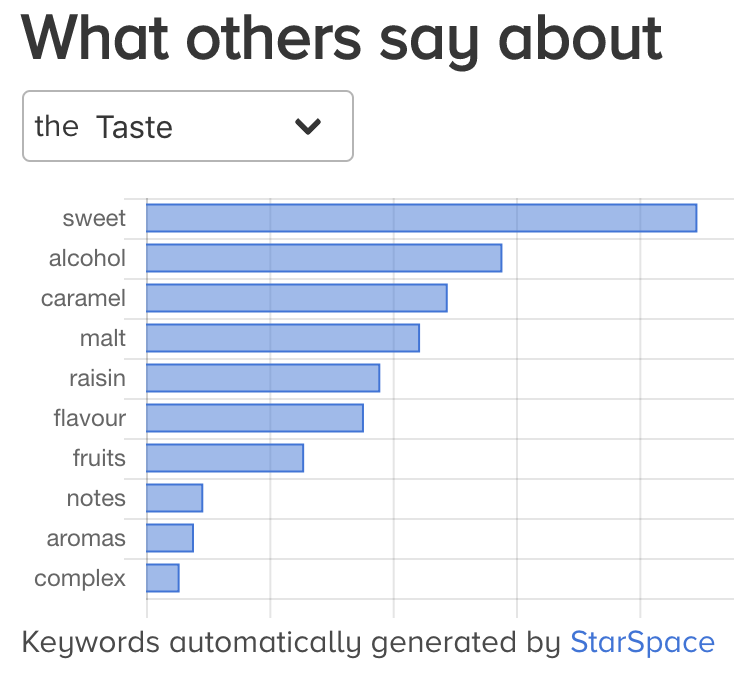
\includegraphics[width=5cm]{assets/beer_keywords.png}
\caption{Nearest neighbor keywords on Beerlytics}
\centering
\label{fig:beer-nn}
\end{figure}

Finally, a map underneath the keyword chart summarizes the distribution places of a beer.
Instead of displaying a marker at the location of each place it dynamically clusters markers in the vicinity of each other.
Zooming into the map breaks up these clusters until only single markers remain.
Clicking on a place marker opens an info-box in the map which renders name and an exemplary image of the place (if available).
Further information about the place appears below the map and includes address, opening times, telephone number, and social media links.